\documentclass[a4paper, 12pt]{report}
\usepackage[italian]{babel}
\usepackage[utf8]{inputenc}
\usepackage{graphicx}
\usepackage{amsmath}

\title{Il problema di Monty Hall}
\author{Robert Octavian Timofte - VR429581}
\date{Maggio 2021}

\begin{document}

\maketitle
\tableofcontents

\chapter*{Introduzione}
Il \textbf{problema di Monty Hall} (o paradosso di Monty Hall) è un famoso problema di teoria della probabilità, legato al gioco a premi statunitense Let's Make a Deal. Prende il nome da quello del conduttore dello show, Maurice Halprin, noto con lo pseudonimo di Monty Hall. Il problema è anche noto come \textbf{paradosso di Monty Hall}, poiché la soluzione può apparire controintuitiva, ma non si tratta di una vera antinomia, in quanto non genera contraddizioni logiche.

Nel gioco vengono mostrate al concorrente tre porte chiuse; dietro ad una si trova un'automobile, mentre ciascuna delle altre due nasconde una capra. Il giocatore può scegliere una delle tre porte, vincendo il premio corrispondente. Dopo che il giocatore ha selezionato una porta, ma non l'ha ancora aperta, il conduttore dello show – che conosce ciò che si trova dietro ogni porta – apre una delle altre due, rivelando una delle due capre, e offre al giocatore la possibilità di cambiare la propria scelta iniziale, passando all'unica porta restante; cambiare la porta migliora le chance del giocatore di vincere l'automobile, portandole da 1/3 a 2/3.

\chapter{Storia del problema e sua soluzione}
\section{Il problema}
Una famosa formulazione del problema è contenuta in una lettera del 1990 di Craig F. Whitaker, indirizzata alla rubrica di Marilyn vos Savant nel settimanale \textit{Parade}:

\begin{quote}
	\textit{Supponi di partecipare a un gioco a premi, in cui puoi scegliere fra tre porte: dietro una di esse c'è un'automobile, dietro le altre, capre. Scegli una porta, diciamo la numero 1, e il conduttore del gioco a premi, che sa cosa si nasconde dietro ciascuna porta, ne apre un'altra, diciamo la 3, rivelando una capra. Quindi ti domanda: "Vorresti scegliere la numero 2?" Ti conviene cambiare la tua scelta originale?}
\end{quote}

Quella proposta sopra è una formulazione del problema data da Steve Selvin, in una lettera all'\textit{American Statistician} (febbraio 1975). Così impostato, il problema è in realtà una variazione sul tema del gioco a premi originale; Monty Hall in effetti apriva una porta dietro cui si trovava una capra per aumentare la tensione, ma non consentiva ai giocatori di cambiare la propria scelta originale. Come scrisse lo stesso Monty Hall a Selvin:

\begin{quote}
	\textit{E se mai dovesse partecipare al mio gioco, le regole sarebbero le stesse per lei - nessuno scambio dopo la scelta originale.}
\end{quote}

Marilyn vos Savant risolse il problema correttamente; l'episodio fece un certo scalpore, in quanto diversi accademici non riconobbero la correttezza della soluzione proposta dalla vos Savant finché questa non la spiegò nel dettaglio in un successivo articolo.

La successiva lettera di Selvin all'\textit{American Statistician} (agosto, 1975) battezza il problema come "Problema di Monty Hall".

Un problema essenzialmente identico appare in ogni modo nella rubrica \textit{Mathematical Games} (sulla rivista Scientific American) di Martin Gardner nel 1959, col nome di "Problema dei tre prigionieri".

Questo problema era stato ideato dal matematico francese Joseph Louis François Bertrand che lo aveva proposto nel suo libro \textit{Calcul des Probabilités} (1889) ed era noto come il Paradosso delle tre scatole di Bertrand.

Quella che segue, per concludere, è una formulazione del problema priva di ambiguità, con vincoli espliciti concernenti il comportamento del conduttore, presentata da Mueser e Granberg:

\begin{itemize}
	\item Dietro ciascuna di tre porte c'è un'automobile o una capra (due capre, un'automobile in tutto); la probabilità che l'automobile si trovi dietro una data porta è identica per tutte le porte;
	\item Il giocatore sceglie una delle porte; il suo contenuto non è rivelato;
	\item Il conduttore sa ciò che si nasconde dietro ciascuna porta;
	\item Il conduttore deve aprire una delle porte non selezionate, e deve offrire al giocatore la possibilità di cambiare la sua scelta;
	\item Il conduttore aprirà sempre una porta che nasconde una capra;
	      \begin{itemize}
		      \item Cioè, se il giocatore ha scelto una porta che nasconde una capra, il conduttore aprirà la porta che nasconde l'altra capra;
		      \item Se invece il giocatore ha scelto la porta che nasconde l'automobile, il conduttore sceglie a caso una delle due porte rimanenti;
	      \end{itemize}
	\item Il conduttore offre al giocatore la possibilità di reclamare ciò che si trova dietro la porta che ha scelto originalmente, o di cambiare, reclamando ciò che si trova dietro la porta rimasta.
\end{itemize}

Le possibilità di vittoria aumentano per il giocatore se cambia la propria scelta?

\section{Soluzione}
La risposta è \textbf{sì}; le probabilità di trovare l'automobile raddoppiano.

La soluzione può essere illustrata come segue. Ci sono tre scenari possibili, ciascuno avente probabilità 1/3:

\begin{itemize}
	\item Il giocatore sceglie la capra numero 1. Il conduttore sceglie l'altra capra, la numero 2. Cambiando, il giocatore vince l'auto.
	\item Il giocatore sceglie la capra numero 2. Il conduttore sceglie l'altra capra, la numero 1. Cambiando, il giocatore vince l'auto.
	\item Il giocatore sceglie l'auto. Il conduttore sceglie una capra, non importa quale. Cambiando, il giocatore trova l'altra capra.
\end{itemize}

Nei primi due scenari, cambiando il giocatore vince l'auto; nel terzo scenario il giocatore che cambia non vince. Dal momento che la strategia "cambiare" porta alla vittoria in due casi su tre, le \textit{chance} di vittoria adottando la strategia sono 2/3.

Indichiamo le porte con A, B e C. Nel caso in cui l'auto sia dietro la porta A la tabella potrebbe essere come la seguente.

\begin{table}[htbp]
	\centering
	\begin{tabular}{|c|l|l|}
		\hline
		\textbf{Porta scelta} & \multicolumn{1}{c|}{\textbf{Il giocatore cambia}} & \multicolumn{1}{c|}{\textbf{Il giocatore non cambia}} \\ \hline
		A                     & Perde                                             & Vince                                                 \\ \hline
		B                     & Vince                                             & Perde                                                 \\ \hline
		C                     & Vince                                             & Perde                                                 \\ \hline
	\end{tabular}
\end{table}

Una strategia di soluzione alternativa è considerare che se si suppone di cambiare, il solo caso in cui si perde è quello in cui originariamente si è scelta l'automobile e quindi la domanda del conduttore può essere considerata un \textit{invito} a invertire le probabilità di successo con quelle di insuccesso.

Il problema sarebbe diverso se non ci fosse una scelta iniziale, o se il conduttore scegliesse una porta a caso, o se il conduttore potesse offrire al giocatore di cambiare a seconda della scelta iniziale del giocatore. Alcune formulazioni del problema, e significativamente quella del settimanale \textit{Parade}, non escludono esplicitamente queste possibilità; diversi testi di probabilità elementare riportano varianti del problema. Per esempio, se il conduttore offre la possibilità di cambiare solo se il giocatore inizialmente ha scelto l'automobile, le \textit{chance} di vittoria associate alla strategia "cambiare" sono, ovviamente, dello 0\%. Nella formulazione proposta nella sezione precedente, il giocatore che cambia ha una probabilità di vittoria pari a 2/3 precisamente perché il conduttore \textbf{deve} offrirgli la possibilità di cambiare, e \textbf{deve} rivelare una capra.

\chapter{Aiuti alla comprensione del problema}
\section{Diagrammi di Eulero-Venn}
La probabilità che l'auto sia dietro la porta restante può essere calcolata con l'ausilio del diagramma di Venn illustrato sotto. Dopo aver scelto la porta 1, per esempio, il giocatore ha probabilità 1/3 di aver selezionato la porta con l'auto, il che assegna una probabilità pari a 2/3 alle due porte restanti. Si osservi che c'è una probabilità pari a 1 di trovare una capra dietro almeno una delle due porte non selezionate dal giocatore, dal momento che c'è una sola auto in palio.

\begin{figure}[h]
	\centering
	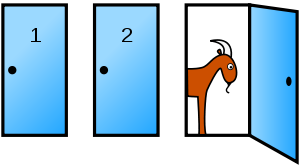
\includegraphics[scale=0.5]{monty1}
\end{figure}

Si supponga che il conduttore apra la porta 3. Dal momento che può solo aprire una porta che nasconde una capra, e non apre una porta a caso, questa informazione non ha effetto sulla probabilità che l'auto sia dietro la porta originariamente selezionata, che resta pari a 1/3. Ma l'auto non è dietro la porta 3, dunque l'intera probabilità di 2/3 delle due porte non selezionate dal giocatore è ora assegnata alla sola porta 2, come mostrato sotto. Un modo alternativo per arrivare a questa conclusione è osservare che se l'auto si trova dietro la porta 2 o dietro la porta 3, aprire la porta 3 implica che l'auto si trova dietro la 2 e viceversa.

\begin{figure}[h]
	\centering
	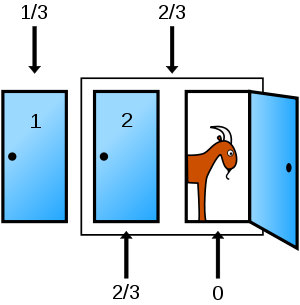
\includegraphics[scale=0.5]{monty2}
\end{figure}

Osserviamo che il problema non cambierebbe se il conduttore, anziché aprire una porta, offrisse al giocatore la possibilità di cambiare la porta scelta con entrambe le altre. In questo caso è evidente che la probabilità è 2/3.

Viceversa, la situazione cambierebbe completamente se il presentatore, dopo aver escluso la porta 3, scambiasse casualmente i premi nascosti dietro le porte 1 e 2. In questo caso il giocatore avrebbe probabilità 1/2 di vincere sia se mantiene la porta 1, sia se la cambia. Senza questo \textit{rimescolamento} le probabilità restano 1/3 e 2/3.

\section{Teorema di Bayes}
Un'analisi del problema attraverso il teorema di Bayes rende esplicito l'effetto delle ipotesi sopra indicate. Si consideri, senza perdere la generalità dell'analisi, il caso in cui la porta 3 è stata aperta dal conduttore mostrando una capra, e che il concorrente abbia selezionato la porta 1.

La probabilità che l'automobile si trovi dietro la porta 2 (ovvero la probabilità di trovare l'auto dopo aver cambiato la scelta iniziale) è \(1-P(A1|C3)\) ove A1 è l'evento che l'auto si trovi dietro alla porta 1 e C3 è l'evento che il conduttore selezioni una capra dietro la porta 3. La probabilità (\textit{a priori}, utilizzando il gergo della statistica bayesiana) che l'automobile si trovi dietro la porta 1, che si denota con \(P(A1)\), è chiaramente 1/3, in quanto l'auto ha \textit{a priori} la stessa probabilità di trovarsi dietro ciascuna porta. La probabilità che il conduttore apra la porta 3 con dietro una capra, \(P(C3)\), è altrettanto chiaramente 1/2 (dal punto di vista del concorrente), visto che il conduttore deve scegliere una delle due porte non scelte dal concorrente. La probabilità che il conduttore selezioni una porta con dietro la capra posto che l'automobile sia dietro la porta 1, \(P(C3|A1)\), è 1/2 perché se l'automobile è dietro la porta 1, scelta inizialmente, il conduttore può scegliere di aprire una delle altre due porte 2 o 3: dal punto di vista del concorrente il conduttore ha quindi due porte tra cui scegliere, cioè probabilità 1/2 per ognuna.

Pertanto, sfruttando il teorema di Bayes:
\newline
La probabilità di trovare l'auto cambiando la scelta iniziale, dopo che il conduttore (onnisciente) ha mostrato una porta con dietro la capra è:

\begin{equation*}
	P(A2|C3) = 1 - P(A1|C3) = 1 - \frac{P(C3|A1)P(A1)}{P(C3)} = 1 - \frac{\frac{1}{2} \times \frac{1}{3}}{\frac{1}{2}} = \frac{2}{3}
\end{equation*}

Oppure, considerando che \(P(C3|A2)=1\) dato che al conduttore non rimane che aprire l'unica porta non scelta dal concorrente con dietro una capra, si può calcolare direttamente:

\begin{equation*}
	P(A2|C3) = \frac{P(C3|A2)P(A2)}{P(C3)} = \frac{1 \times \frac{1}{3}}{\frac{1}{2}} = \frac{2}{3}
\end{equation*}

\section{Teorema delle probabilità totali}
Dimostriamo ora che, cambiando sempre l'ultima scelta, la probabilità di vincere l'automobile è \(\frac{2}{3}\) mediante il teorema delle probabilità totali. Ricordiamo che la nostra strategia è di scegliere mentalmente due porte, di indicare al conduttore l'altra porta e poi di cambiare. Indichiamo con \(V\) l'evento "vittoria seguendo questa strategia". Sia \(A\) l'evento "sotto le due porte scelte mentalmente c'è la macchina" e \(B\) l'evento complementare.

Chiaramente \(P(A)=\frac {2}{3}\). Si noti anche che \(P(V|A) = 1\) poiché, grazie alla strategia scelta, se la macchina si trova dietro le due porte scelte mentalmente, il conduttore ci indicherà poi quella vincente aprendo la porta perdente. Per il teorema delle probabilità totali abbiamo allora

\begin{equation*}
	P(V) = P(V|A)P(A) + P(V|B)P(B) = 1 \times \frac{2}{3} + 0 \times \frac{1}{3} = \frac{2}{3}
\end{equation*}

\chapter{Varianti}
\section{Il conduttore non sa cosa ci sia dietro le porte}
Dopo la scelta del concorrente, il conduttore apre una delle due porte rimaste. Poiché non sa cosa c'è dietro, con probabilità 1/3 trova l'auto e il gioco finisce. Con probabilità 2/3 trova invece la capra e può chiedere al concorrente se vuole effettuare il cambio con la porta rimasta chiusa. In questo caso accettare lo scambio non fa aumentare al concorrente la sua probabilità di vincere che a questo punto è di 1/2 qualunque sia la sua decisione.

\section{Due giocatori}
Ad alcuni minuti dalla fine del gioco, il conduttore sceglie due concorrenti a cui proporre "la grande scommessa". Dietro a una delle tre porte c'è il premio più consistente. Ad ogni giocatore è permesso scegliere una porta (non la stessa).

In questo scenario, si può esaminare una variante del problema. Il presentatore elimina il giocatore che abbia scelto una porta con dietro la capra (se lo hanno fatto entrambi, ne viene scelto uno a caso), apre la porta, svelando la capra e poi offre al giocatore rimanente la possibilità di cambiare la propria scelta. Il giocatore dovrebbe effettuare lo scambio?

La risposta è \textit{no}. La ragione: il giocatore che effettuasse lo scambio in questo tipo di gioco vincerebbe se e solo se entrambi i giocatori avessero scelto una porta con la capra. che probabilità ha questa evenienza? 1/3. Se mantenesse la scelta resterebbero 2/3 di probabilità. Quindi chi mantenesse la scelta fatta inizialmente avrebbe il doppio delle possibilità di vincere.

In alternativa, ci sono tre possibili scenari, tutti con uguale probabilità (1/3):

\begin{itemize}
	\item Il giocatore 1 sceglie la porta che nasconde l'auto. Il conduttore deve eliminare il giocatore 2. Cambiare scelta comporta perdere.
	\item Il giocatore 2 sceglie la porta che nasconde l'auto. Il conduttore deve eliminare il giocatore 1. Cambiare scelta comporta perdere.
	\item Nessuno dei giocatori sceglie la porta che nasconde l'auto. Il conduttore elimina a caso uno dei due giocatori. Cambiare scelta comporta vincere.
\end{itemize}

Il giocatore 1 è l'unico rimasto nel primo caso, e lo è con probabilità 1/2 nel terzo caso; in questa eventualità cambiare scelta comporta una probabilità di perdere (1/3) due volte maggiore di quella di vincere (1/6). Analogamente, nel secondo caso il giocatore 2 è l'unico rimasto, e lo è con probabilità 1/2 nel terzo caso; in questa eventualità cambiare scelta comporta una probabilità di perdere (1/3) due volte maggiore di quella di vincere (1/6). Dunque a prescindere da quale giocatore rimanga, c'è una probabilità pari a 2/3 di vincere se non si cambia scelta. Per rendere più palese la differenza rispetto al caso precedente si può dire che non si può qui ragionare come prima dove il (solo) giocatore arriva sempre al secondo turno (quello del possibile scambio) e la probabilità che abbia selezionato la scelta vincente rimane 1/3, contro i complementari 2/3 della scelta alternativa. Si deve invece notare che nell'istante in cui un giocatore (uno dei due) arriva al secondo turno deve considerare che la probabilità che abbia inizialmente effettuato la scelta giusta si modifica e sale a 2/3. In sostanza il giocatore rimasto riveste in questo caso, in termini di probabilità, lo stesso ruolo che prima (caso con un giocatore) ricopriva la porta non selezionata dal giocatore né eliminata dal conduttore.

\section{\textit{n} porte}
Esiste una generalizzazione del problema originale in cui si hanno \textit{n} porte: nel primo stadio del gioco, il giocatore sceglie una porta. Quindi il conduttore apre un'altra porta, che nasconde una capra. Se il giocatore vuole, può quindi cambiare scelta e passare a un'altra porta. Il conduttore aprirà allora un'ulteriore porta, ancora non aperta, che nasconde una capra, diversa da quella attualmente scelta dal giocatore. Il giocatore ha quindi la possibilità di cambiare ancora scelta, e così via. Questo procedimento continua fino a che non restano che due porte non ancora aperte: la scelta corrente del giocatore, e un'altra porta. Quante volte dovrebbe cambiare scelta il giocatore, e a che punto del gioco (sempre che cambi almeno una volta)?

La migliore strategia è: \textit{restare con la prima scelta sino a che non rimangano solo due porte e a quel punto cambiare}. Seguendo questa strategia la probabilità di vincere è \((n-1)/n\). Questa variante del paradosso di Monty Hall si deve a Bapeswara Rao e Rao.

\section{Variante nel gioco del bridge}
Una comune variante del problema è nota ai giocatori di bridge da ben prima che l'articolo della Vos Savant fosse pubblicato. Tale variante è nota come principio della scelta ristretta.

\section{Versione quantistica}
Esiste una versione quantistica del paradosso, che illustra alcuni aspetti della relazione tra la teoria dell'informazione classica (non quantistica) e l'informazione quantistica, ossia l'informazione codificata negli stati di sistemi meccanici quantistici. Le tre porte sono rimpiazzate da un sistema quantistico che consta di tre alternative, in cui aprire una porta e vedere cosa nasconde si traduce in fare una particolare misurazione. Le regole del gioco possono essere espresse in questo linguaggio, e ancora una volta il giocatore può scegliere se restare fedele alla propria scelta iniziale o cambiare e optare per una scelta alternativa ("ortogonale"). Quest'ultima strategia ha probabilità di vittoria doppie, esattamente come nel caso classico. Tuttavia, se la posizione del premio non è pienamente casuale in senso quantistico, il giocatore può fare ancora meglio, e in determinati casi vincere con probabilità pari a uno.

\section{Spiegazione caso per caso}
Poiché in questo gioco i casi possibili non sono molti, si può pensare di schematizzarli come segue, raggruppandoli seguendo la scelta della porta iniziale:
\newline
\textit{Scelgo la porta A}
\begin{enumerate}
	\item \textbf{G}GC $\rightarrow$ (M apre la 2) $\rightarrow$ \textbf{G}XC $\rightarrow$ resto-perdo, cambio-vinco
	\item \textbf{G}CG $\rightarrow$ (M apre la 3) $\rightarrow$ \textbf{G}CX $\rightarrow$ resto-perdo, cambio-vinco
	\item \textbf{C}GG $\rightarrow$ (M apre la 2 o la 3) $\rightarrow$ \textbf{G}XC o \textbf{C}GX $\rightarrow$ resto-vinco, cambio-perdo
\end{enumerate}
\textit{Scelgo la porta B}
\begin{enumerate}
	\item G\textbf{G}C $\rightarrow$ (M apre la 1) $\rightarrow$ X\textbf{G}C $\rightarrow$ resto-perdo, cambio-vinco
	\item G\textbf{C}G $\rightarrow$ (M apre la 1 o la 3) $\rightarrow$ X\textbf{C}G o G\textbf{C}X $\rightarrow$ resto-vinco, cambio-perdo
	\item C\textbf{G}G $\rightarrow$ (M apre la 3) $\rightarrow$ C\textbf{G}X $\rightarrow$ resto-perdo, cambio-vinco
\end{enumerate}
\textit{Scelgo la porta C}
\begin{enumerate}
	\item GG\textbf{C} $\rightarrow$ (M apre la 1 o la 2) $\rightarrow$ XG\textbf{C} o GX\textbf{C} $\rightarrow$ resto-vinco, cambio-perdo
	\item GC\textbf{G} $\rightarrow$ (M apre la 1) $\rightarrow$ XC\textbf{G} $\rightarrow$ resto-perdo, cambio-vinco
	\item CG\textbf{G} $\rightarrow$ (M apre la 2) $\rightarrow$ CX\textbf{G} $\rightarrow$ resto-perdo, cambio-vinco
\end{enumerate}

Le disposizioni in elenco numerate da uno a tre sono le configurazioni in cui si possono trovare disposte le due capre (G=Goat) e l'auto (C=Car) dietro ciascuna porta (A, B o C) all'inizio del gioco. Ovviamente non cambiano al cambiare della prima scelta del concorrente e sono a lui del tutto ignote. Dopo tale scelta iniziale, il conduttore (M=Monty) apre una delle due porte che nascondono le capre, cosicché rimangono due porte chiuse, cioè quella inizialmente scelta e l'ultima da aprire: ad esempio, in caso di scelta della porta A ed in presenza della disposizione 1, avremo il caso iniziale \textbf{G}GC (in cui il grassetto indica la porta scelta), dove Monty sarà costretto a rivelare la capra dietro la porta B, cioè, indicando con X la porta aperta non più in gioco, ci troveremo nel caso \textbf{G}XC. In questo caso, se il concorrente rimane sulla propria scelta iniziale (resto), perde.

Come si può notare semplicemente contando i casi vincenti relativi ad ogni modalità di gioco, cioè qualsiasi porta inizialmente lui scelga e considerando le tre disposizioni possibili, ne esistono due su tre favorevoli al concorrente che corrispondono al cambiare la scelta iniziale.

\end{document}